\documentclass[../Book.Stress_regulation.tex]{subfiles}
\graphicspath{{\subfix{../images/}}}
\begin{document}

\epigraph{Pleasure in the job puts perfection in the work.}{\textit{Aristotle}}

\subsubsection{Stress Hormones}


During stress, the so called stress hormones\index{stress hormones} get released in our body: \emph{Noradrenaline} and \emph{Adrenaline}.
Their job is to provide as much {energy} in the from of sugar from the liver to the body, as fast as possible.
The fastest acting one is Noradrenaline\index{stress hormones!Noradrenaline}, which readies our body for the incoming stressful situation.


% ------------------------------------------------


\subsubsection{Noradrenaline vs. Adrenaline}

\begin{figure}[htb]
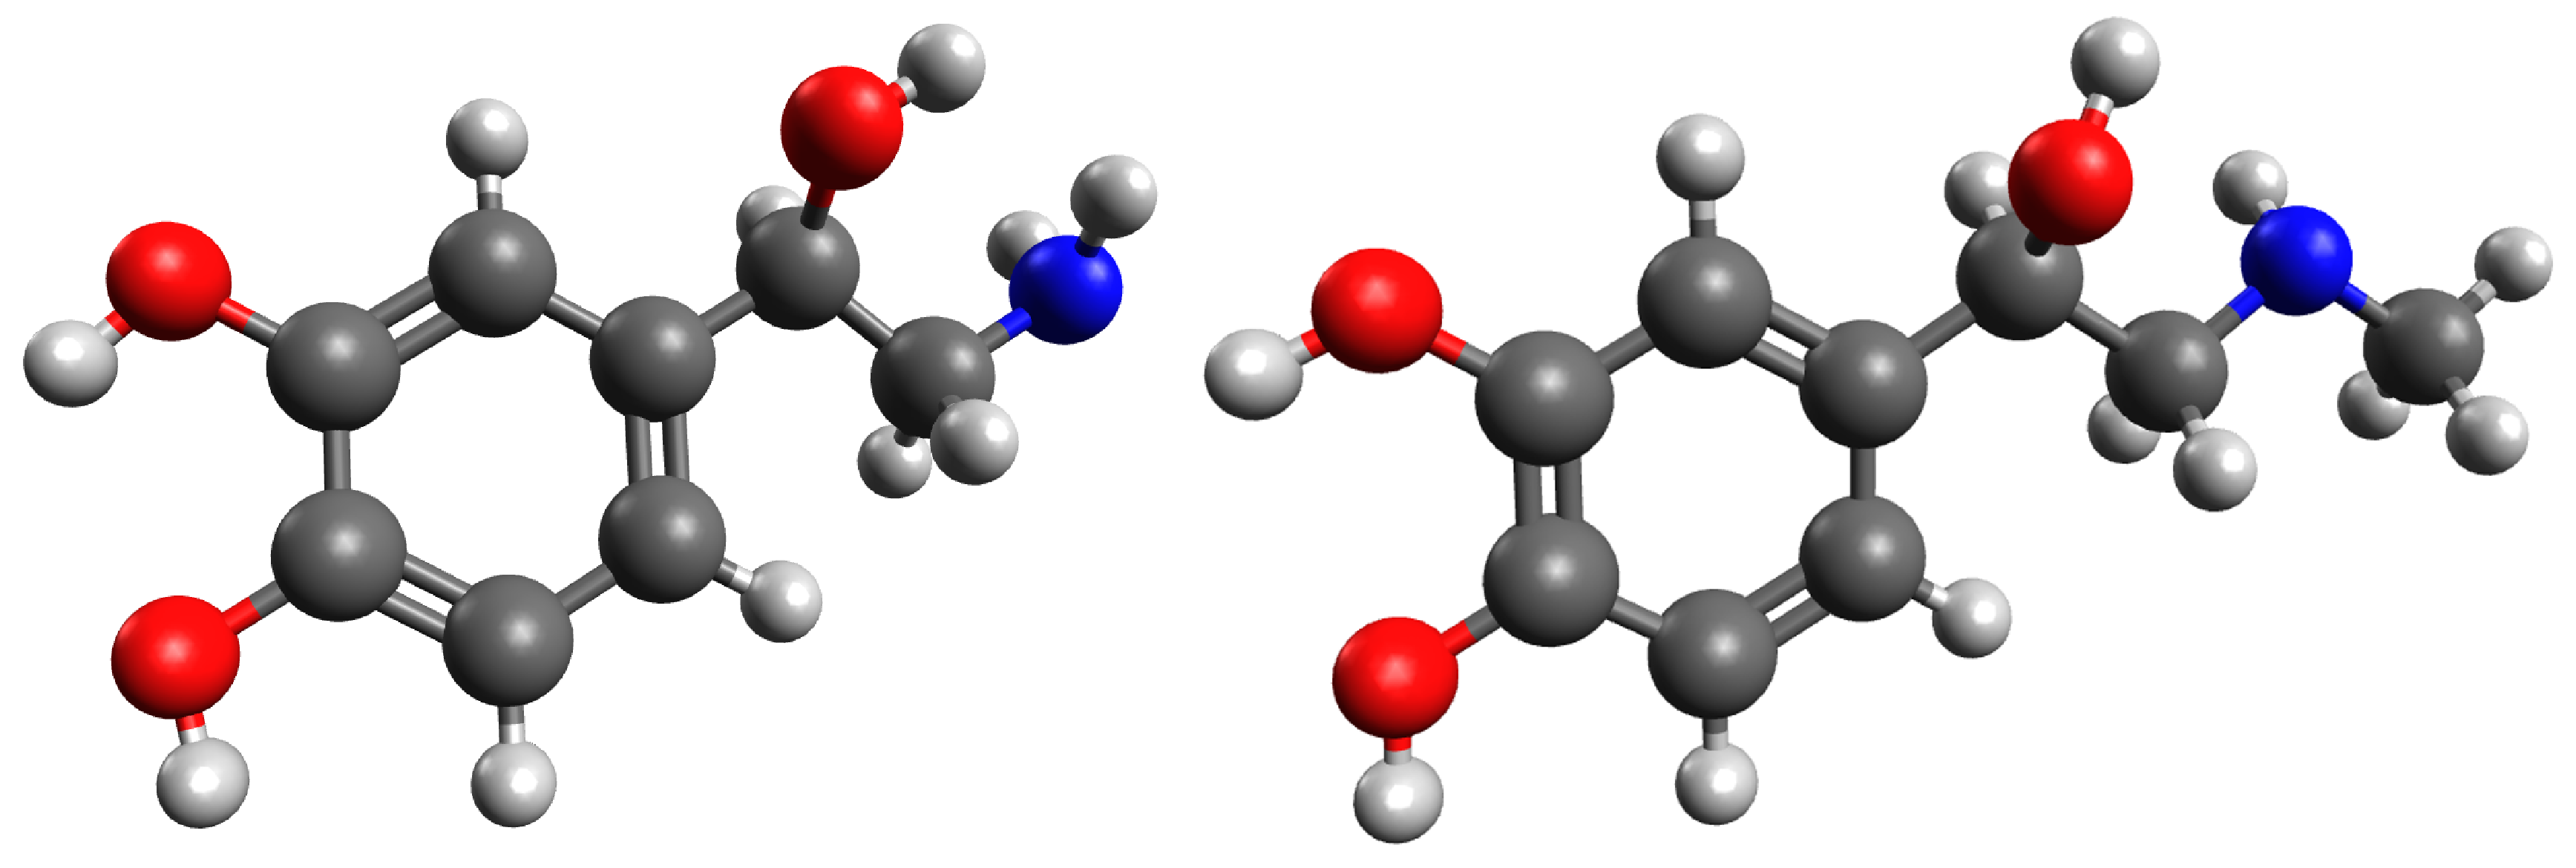
\includegraphics[width=12cm]{Nor_Adrenaline}
\caption{The structures of Noradrenaline and Adrenaline}
\end{figure}

Noradrenaline has it's {own release system} in the body. It gets released by free nerve endings of the somatic nervous system\index{nervous system!somatic}.
The somatic nerves are the nerves situated in our body as opposed to in the central nervous system.
It bypasses the slower blood stream transport system. Noradrenaline prepares us in a {``cool'' way} for danger, by providing muscles instantaneously with energy in the form of glucose (sugar).
The actions of Noradrenaline doesn't get noticed by the hearth, so the hearth rate doesn't get affected yet.
Both, eustress and distress cause the release of catecholamines\footnote{Catecholamines is a medical expression, most often used in it's plural form, catecholamines. Another name is Brenzcatechineamines. They are a class of body's own and synthetic chemical compounds, which have a stimulating effect at the sympathetic alpha and beta receptors of the hearth--circulation. Therefore catecholamines are sympathomimetics. They all have a similar structure and are related to phenylethylamines and substances related to adrenaline.}, Noradrenaline (over the somatic nervous system\footnote{The nervous system of the body, as opposed to the central nervous system.}) and Adrenaline (over the bloodstream) gets released.



\subsubsection{The Typical Stress Reaction}
The ``typical'' stress reaction doesn't exist, it's a \emph{process}: the body tries to get back into {equilibrium} after an irritating stimulus, which can be perceived as positive or negative.
The emotions going along with this aren't uniform.
They depend on the {personality structure}\index{personality!structure} and the {intensity} of the of the experiencing.

But what is for sure is that every burden which hits us and which we don't {consciously acknowledge} will express itself sooner or later by the means of the body.

\end{document}

